\documentclass[11pt,class=report,crop=false]{standalone}
\usepackage[screen]{../python}

\begin{document}

\setcounter{section}{0}

%====================================================================
\chapter*{Annexe}
%====================================================================
\addcontentsline{toc}{chapter}{Annexe}

\objectifs{On regroupe ici quelques informations diverses et variées.}


%%%%%%%%%%%%%%%%%%%%%%%%%%%%%%%%%%%%%%%%%%%%%%%%%%%%%%%%%%%%%%%%%%%%%
\section{Une brève histoire des réseaux de neurones}

\begin{itemize}
  \item \textbf{Neurone en biologie.} Entre 1840 et 1900 on découvre que la cellule est l'élément fondamental du vivant ; par observation, Santiago Ram\'on y Cajal et d'autres mettent en évidence que les cellules du système nerveux forment un réseau : les neurones.
  On sait maintenant que le cerveau humain contient entre 80 et 100 milliards de neurones, mais nous avons aussi 500 millions de neurones dans le ventre (soit autant que dans le cerveau d'un chien).
  Un neurone est composé d'un élément central prolongé par un axone au bout duquel se trouvent les synapses. Les neurones sont organisés en réseau, un neurone étant en moyenne relié à $10\,000$ autres neurones et transmet ainsi un signal électrique à tous ses neurones voisins. 
    
  \item \textbf{De la biologie vers l'informatique.} À la fin des années 1940, Donald Hebb  émet l'hypothèse que lors de l'apprentissage certaines connexions synaptiques se renforcent et que ce renforcement persiste. Un modèle mathématique est déduit par Frank Rosenblatt : le perceptron (1958). L'algorithme est mis en \oe uvre dans une machine dédiée à la reconnaissance d'images. 
  Le perceptron, qui correspond à un réseau formé d'un seul neurone, montre très vite ses limites à la fois théoriques (puisqu'il ne peut réaliser le \og{}ou exclusif\fg{}) et aussi en termes de résultats pratiques. Ces deux problèmes sont résolus en considérant des réseaux à plusieurs couches,  mais les calculs à mener sont trop longs à la fois en raison de la puissance des ordinateurs de l'époque et des algorithmes utilisés.  
  
  \item \textbf{Rétropropagation.} Un progrès important est fait grâce l'algorithme de rétropropagation (par Rumelhart, Hinton et Williams en 1986) qui permet un calcul efficace des poids des neurones. On conserve encore aujourd'hui ce principe : des calculs essentiellement numériques, avec un minimum de calculs symboliques au niveau de chaque neurone (afin de calculer la dérivée), le tout avec un grand nombre d'itérations. Des améliorations se succèdent : pooling, dropout, calculs en parallèle, meilleures descentes de gradient.
  
  \item \textbf{Hiver.} Cependant les attentes de l'intelligence artificielle (peut être le nom a-t-il été mal choisi ?) sont largement déçues car ses applications restent limitées. L'intérêt des scientifiques diminue drastiquement. De 1980 à 2000 on parle de l'hiver de l'intelligence artificielle.
  
  \item \textbf{\emph{Deep learning}.} À partir des années 2000 et surtout après 2010 les réseaux de neurones font des progrès fulgurants grâce à l'apprentissage profond. Yann Le Cun démontre l'efficacité des couches de convolution pour la reconnaissance des chiffres. On réalise et entraîne alors des réseaux ayant de plus en plus de couches grâce à des progrès matériels (par exemple le calcul sur les processeurs graphiques GPU) mais surtout grâce aux couches de convolution qui extraient des caractéristiques abstraites des images.  
  
  \item \textbf{Présent et avenir.} Les réseaux de neurones s'appliquent à de nombreux domaines : la reconnaissance d'images (par exemple la détection de cancer sur une radiographie), les transports (par exemple la conduite autonome des voitures), les jeux (les ordinateurs battent les champions du monde d'échecs, de go et des jeux vidéos les plus complexes), l'écriture (classement, résumé, traduction)\ldots{} 
  Il persiste cependant une certaine méfiance vis à vis des décisions prises par une machine (sentence de justice, diagnostic médical, publicité ciblée). Une meilleure compréhension du fonctionnement des réseaux de neurones par tous est donc indispensable !
\end{itemize}


%%%%%%%%%%%%%%%%%%%%%%%%%%%%%%%%%%%%%%%%%%%%%%%%%%%%%%%%%%%%%%%%%%%%%
\section{Références}

\begin{itemize}
  \item \tensorflow{} est développé par \emph{Google}. De nombreux tutoriels sont disponibles pour les débutants :
  \mycenterline{\href{https://www.tensorflow.org/}{tensorflow.org}}
  
  \item \keras{} est maintenant intégré à \tensorflow{} et facilite sa prise en main. 
  Il a été développé par François Cholet auteur du livre \emph{Deep learning with Python} (Manning publications, 2017). Il y a de nombreux exemples d'application :
  \mycenterline{\href{https://keras.io/}{keras.io}}
  
  \item Le livre \emph{Deep learning/L'apprentissage profond} par Goodfellow, Bengio, Courville contient des concepts plus avancés. Il est disponible en anglais et en français. Une version gratuite est consultable ici :
  \mycenterline{\href{https://www.deeplearningbook.org/}{deeplearningbook.org}}
 
  \item Vous pouvez récupérer l'intégralité des codes \Python{} ainsi que tous les fichiers sources sur la page \emph{GitHub} d'Exo7 :
  \href{https://github.com/exo7math/deepmath-exo7}{\og{}GitHub : Deepmath\fg{}}.
  
  En particulier vous trouvez sur ce site le module \ci{keras_facile} qui vous aide à définir facilement des poids pour un réseau simple.
  
  
  
  \item Un peu de pub pour les livres Exo7 :  
  \begin{itemize}
    \item \emph{Algèbre} et \emph{Analyse} pour toutes les notions de mathématiques niveau première année d'études supérieures,
    \item \emph{Python au lycée} (tome 1 et tome 2) pour apprendre la programmation.
  \end{itemize}
  Ils sont disponibles gratuitement en téléchargement :
  \mycenterline{
  \href{http://exo7.emath.fr/}{exo7.emath.fr} 
  \quad et \quad \href{https://github.com/exo7math/deepmath-exo7}{GitHub : exo7math} 
  }
  et aussi en vente à prix coûtant sur \href{https://www.amazon.fr/}{amazon.fr} en version imprimée.
\end{itemize}



%%%%%%%%%%%%%%%%%%%%%%%%%%%%%%%%%%%%%%%%%%%%%%%%%%%%%%%%%%%%%%%%%%%%%
\section{Ce qu'il faut pour utiliser tensorflow/keras}

Les activités de ce livre sont écrite pour \Python{}, version 3.
Cependant il faut installer un certain nombre de modules complémentaires qui ne sont pas nécessairement présents par défaut.
\begin{itemize}
  \item \ci{tensorflow} qui contient le sous-module \ci{keras},
  \item \ci{numpy} pour les tableaux,
  \item \ci{matplotlib} pour l'affichage de graphiques,
  \item \ci{scipy} pour la convolution,  
  \item \ci{ioimage} pour gérer la lecture et l'écriture d'images.
 
\end{itemize}  

Un module s'installe simplement par :
\mycenterline{\ci{pip install mon_module}}


Il existe des distributions \Python{} (du type \ci{conda}) qui contiennent les principaux modules scientifiques et permettent aussi de créer des \og{}environnements\fg{} afin de gérer plusieurs versions
de \Python{} et de ses modules.

Pour ceux qui souhaitent ne rien installer, il est possible d'utiliser \tensorflow{} en ligne :
\mycenterline{\href{https://colab.research.google.com/notebooks/welcome.ipynb}{Google Colab}}



%%%%%%%%%%%%%%%%%%%%%%%%%%%%%%%%%%%%%%%%%%%%%%%%%%%%%%%%%%%%%%%%%%%%%
\section{Lexique français/anglais}

La plupart des références à propos des réseaux de neurones sont en anglais. Voici donc un petit lexique français/anglais des termes principaux.

\textbf{Réseau de neurones.} \emph{Neural network.}

\begin{itemize}
  \item neurone artificiel/\emph{artificial neuron}
  \item poids/\emph{weights}, biais/\emph{bias}
  \item fonction d'activation/\emph{activation function}
  \item fonction marche de Heaviside/\emph{Heaviside step function}
  \item fonction sigma $\sigma$ ou sigmoïde/\emph{sigmoid function}
  \item fonction d'erreur/\emph{loss function} ou \emph{cost function}
  \item entrée/\emph{input}, sortie/\emph{output}
  \item couches du réseau/\emph{layers}
  \item réseau de neurones avec convolution/\emph{convolutional neural network} abrégé en \emph{cnn}
  \item un motif de convolution s'appelle aussi noyau/\emph{kernel} ou filtre/\emph{filter}
 ou masque/\emph{mask}
  \item \emph{dropout} se traduit par abandon ou décrochage
  \item \emph{pooling} se traduit par regroupement de termes
\end{itemize} 
 
\medskip

\textbf{Mathématiques.}

\begin{itemize}
  \item dérivée partielle/\emph{partial derivative}
  \item gradient/\emph{gradient} mais la notation anglo-saxonne de $\grad f(x,y)$ est $\nabla f(x,y)$
  \item régression linéaire/\emph{linear regression}
  \item tensor/\emph{tensor}, taille/\emph{shape}, nombre d'éléments/\emph{size}
\end{itemize} 
 
 
\medskip
 
\textbf{Descente de gradient.} \emph{Gradient descent.}

\begin{itemize}
 \item descente de gradient (classique)/\emph{(batch) gradient descent}
 \item descente de gradient stochastique/\emph{stochastic gradient descent} abrégée en \emph{sgd}
 \item descente de gradient par lots/\emph{mini-batch gradient descent}
 \item pas $\delta$/\emph{learning rate}
 \item erreur quadratique moyenne/\emph{minimal squared error} abrégée en \emph{mse}
 \item moment/\emph{momentum}
 \item époque/\emph{epoch}
\end{itemize}  

%%%%%%%%%%%%%%%%%%%%%%%%%%%%%%%%%%%%%%%%%%%%%%%%%%%%%%%%%%%%%%%%%%%%%
\section{L'image de couverture}

L'image de couverture du livre est générée automatiquement grâce à un réseau de neurones et  la rétropropagation. Au départ il faut deux images :
\begin{itemize}
  \item une image dont on veut conserver le contenu :  ici la statue de la liberté,
  \item et une image dont on veut conserver le style : ici un tableau de Van Gogh.
\end{itemize}
L'image obtenue possède le contenu de la première et le style de la seconde !

\begin{center}
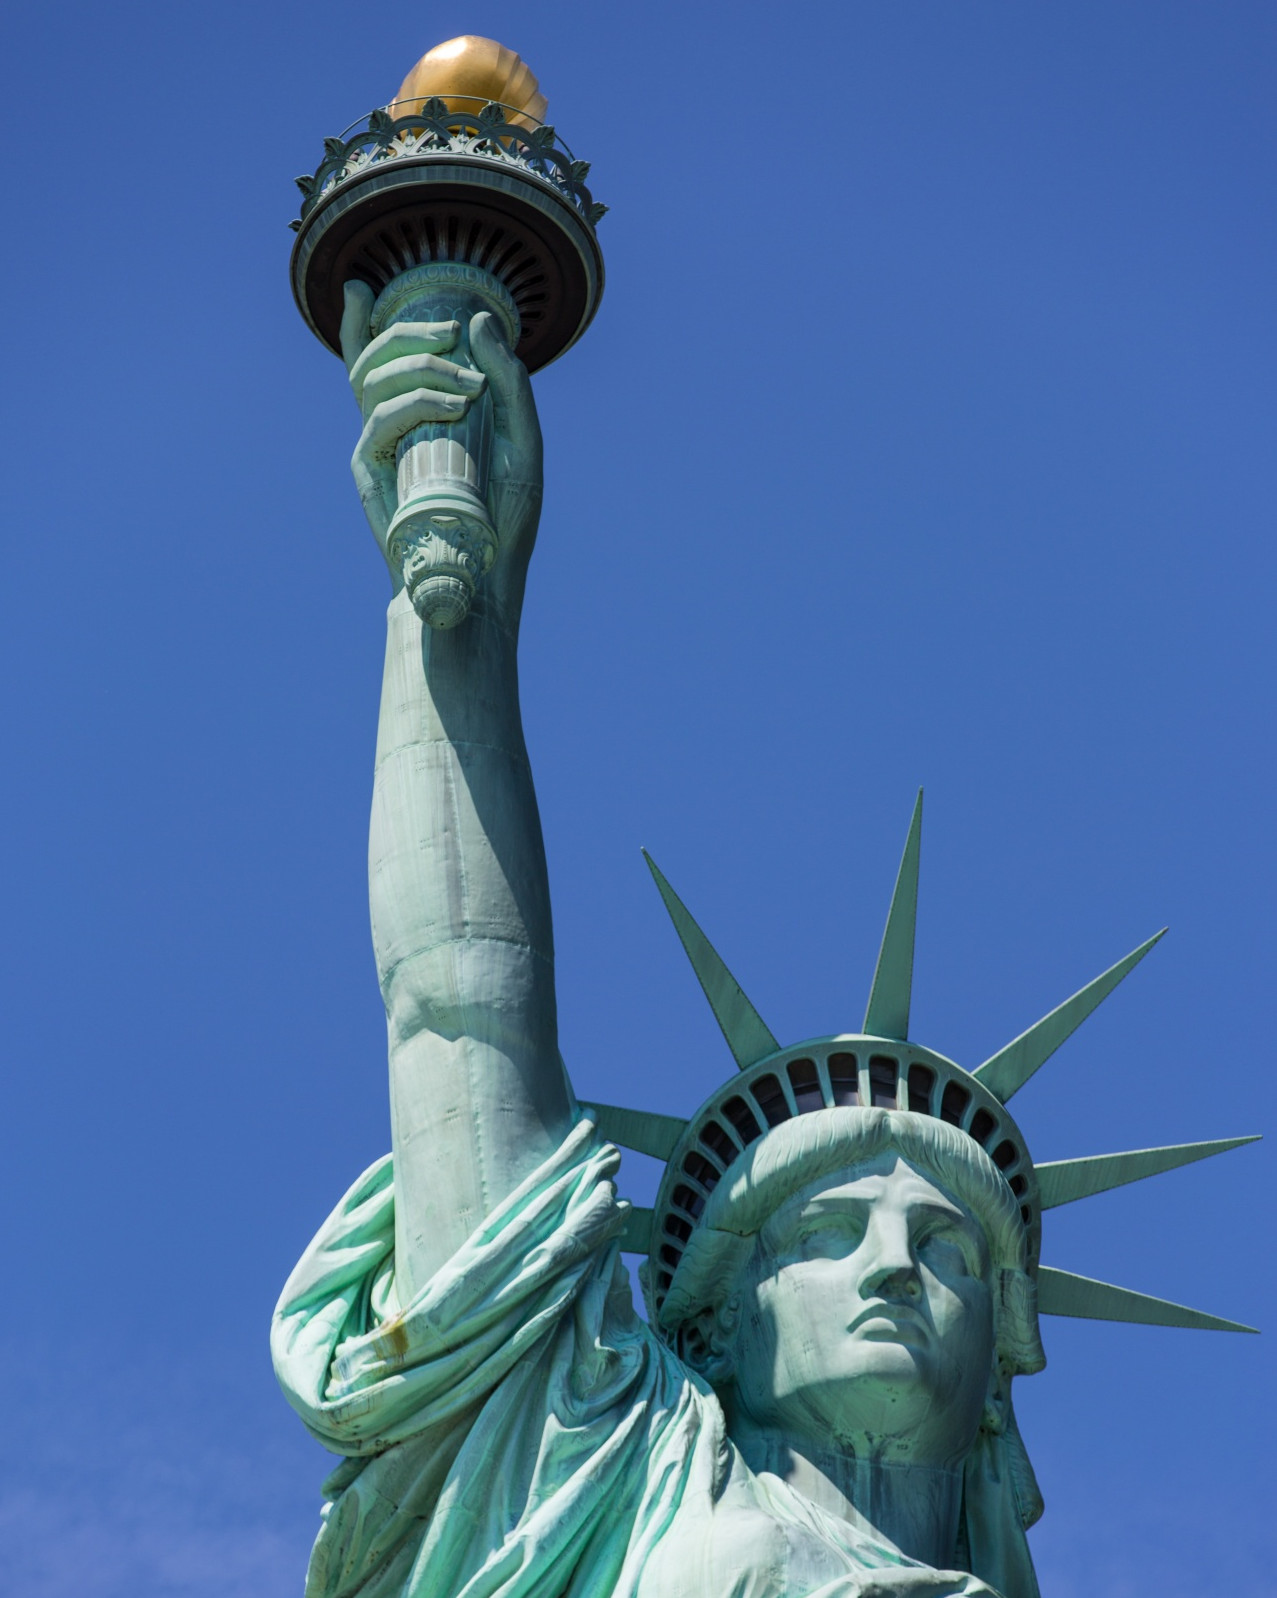
\includegraphics[scale=\myscale,scale=0.15]{figures/statue-of-liberty_resized.jpg}
\qquad\qquad
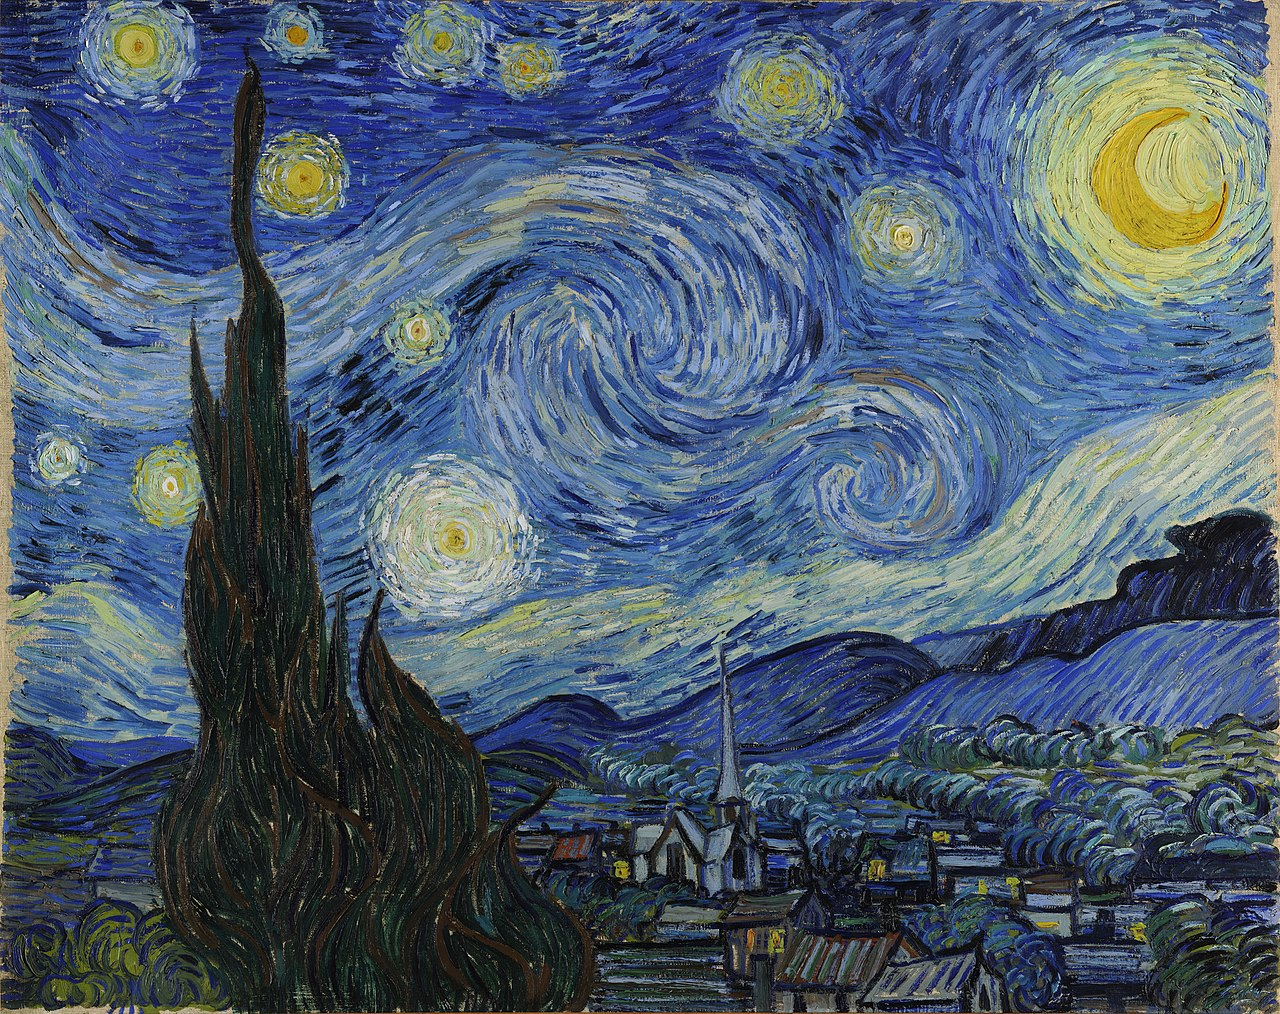
\includegraphics[scale=\myscale,scale=0.18]{figures/Van_Gogh_nuit.jpg}
\end{center}

Références :
\begin{itemize}
  \item Statue de la liberté (photographie par George Hodan, licence CC0, domaine public).
  \item Peinture de Vincent Van Gogh, \emph{La nuit étoilée}, 1889.
  \item Le programme et les explications pour \tensorflow{} :  \href{https://github.com/tensorflow/models/blob/master/research/nst_blogpost/4_Neural_Style_Transfer_with_Eager_Execution.ipynb}{\emph{Neural Style Transfer} avec TensorFlow} d'après des travaux de Gatys, Ecker et Bethge.
\end{itemize}

\begin{center}
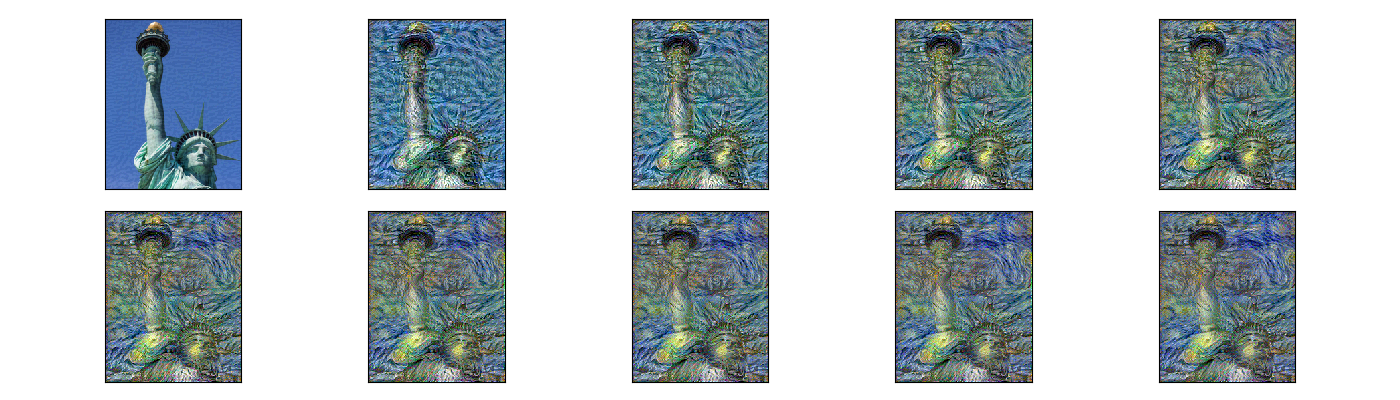
\includegraphics[scale=\myscale,scale=0.5]{figures/iter_500it_256px.png}
\end{center}



Plus en détails :
\begin{itemize}
  \item le réseau de neurones, nommé \og{}VGG19\fg{}, est un réseau à 19 couches. 
  On ne va pas calculer les poids, mais on utilise des poids qui ont déjà été calculés pour reconnaître les images de la base \emph{ImageNet}.
  
  \item Dans ce réseau bien paramétré certaines couches se concentrent sur le contenu (contour, lignes, formes\ldots) et d'autres se concentrent sur le style (couleur, flou\ldots).
  
  \item En identifiant ces couches, on construit par itérations une image qui conserve le contenu de la première image et prend peu à peu le style de la seconde.
  
  \item Ces itérations se font par rétropropagation et descente de gradient selon une fonction d'erreur qui est la somme d'une fonction d'erreur associée au contenu et d'une fonction d'erreur associée au style.
 
\end{itemize}


\begin{center}
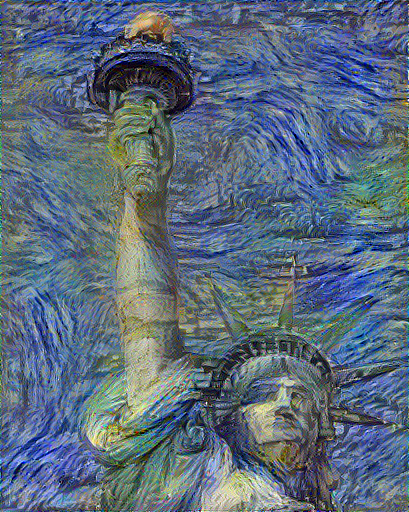
\includegraphics[scale=\myscale,scale=0.5]{figures/best_1000it_512px.png}
\end{center}


\end{document}
